\subsection{Transcriptional Changes to Bovine \textit{IFITs}}
\subsubsection{Responses of bovine cell lines to know activators of innate immune response} \label{Responses of bovine cell lines to know activators of innate immune response}


\subsubsection{Responses of MDBK to bRSV}




\subsubsection{Validation in BT} \label{Validation in BT}
Describe data: \newline
asdasdas

Validation in more physiologically relevant cell line. All genes but bIFIT2 respond to bIFN alpha 5 ng/mL for 3h; treatment for 24h cause no change in any of the genes; treatment for 6h downregulates IFITs but not bMx1. This shows that BT cells are responsive to IFN and have the capability to express bIFITs and bMx1.

Ultracentrifugation purified hRSV causes downregulation in IFITs but not bMx1 (where it causes no change), while infection with normally extracted hRSV cause no change in none of the genes tested. Infections with wt bRSV and dSH bRSV at the same MOI and HPI (1 and 24) cause slight downregulation in all genes tested.

The trends seen with MDBK are kind of recapitulated.

\begin{figure}
    \centering
    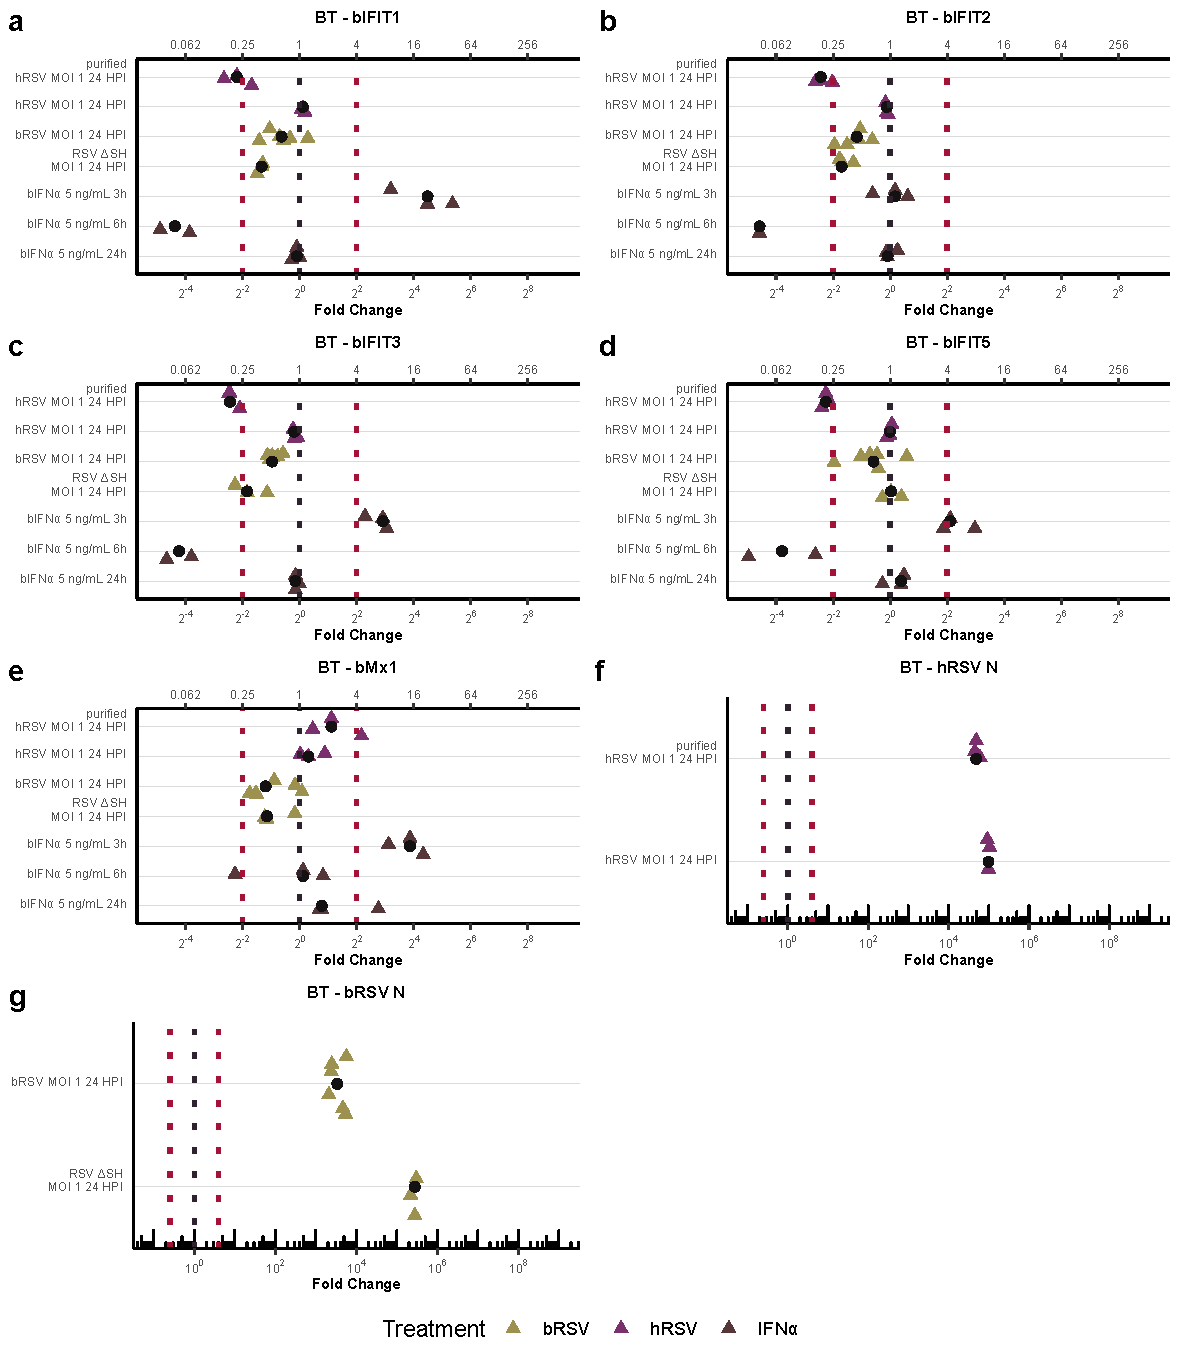
\includegraphics[width=1\linewidth]{07. Chapter 2//Figs/08. bt_plots.pdf}
    \caption[ Validation of bIFIT responses in BT cell line.]{\textbf{ Validation of bIFIT responses in BT cell line.} asdf asdf asds fasdf asdf a sdf asdf asdf asdf as dfas ddf asdf asd}
    \label{ Validation of bIFIT responses in BT cell line}
\end{figure}

\subsubsection{Validation by analysing bRSV RNAseq dataset} \label{Validation by analysing bRSV RNAseq dataset}
Describe data: \newline
asdasdas \newline
Data showing that bIFITs are not differentially expressed in cells infected with dSH bRSV.

This is a dataset that was present in Dalan’s group. Comparing responses at 16 and 40 HPI between WT bRSV vs Mock and dSH bRSV vs Mock. The dataset was previously analysed by a bioinformatician in Pirbright which yield 0 differentially expressed host genes. He however included viral genes in the analysis, which I assume affected the adjusted p values of the host genes due to the relative viral genes abundance. We tried to get in touch with him to discuss this but after several emails got no response. The re-analysis was done on raw annotated count data which had viral transcripts removed. Original analysis was done using EdgeR package, my re-analysis was with DESeq2 (both are valid way of doing DE analysis, EdgeR is more modular and harder to use).

Two volcanos

\begin{figure}
    \centering
    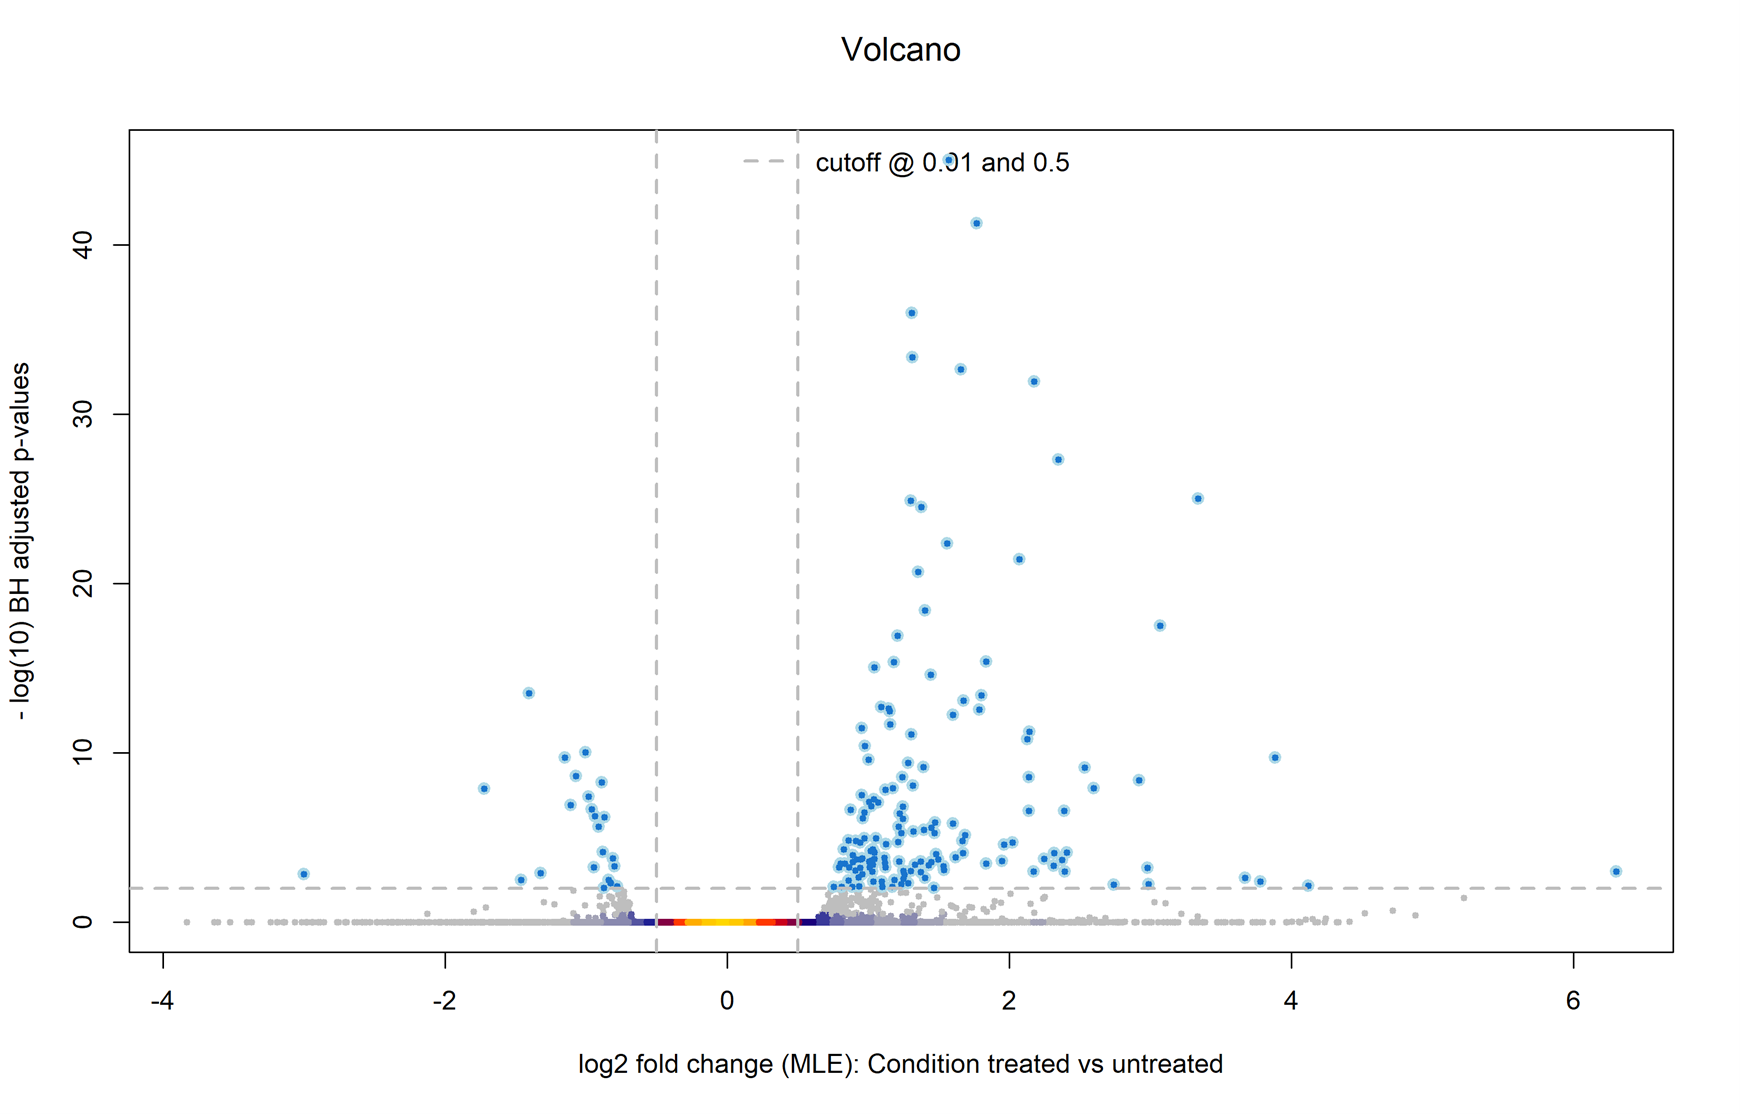
\includegraphics[width=1\linewidth]{07. Chapter 2//Figs/14. rnaseq volcano.png}
    \caption[Volcano plot of DE genes in WT vs Mock 40 HPI.]{\textbf{Volcano plot of DE genes in WT vs Mock 40 HPI.} asdf asdf asdf asdf asdf asdf asdf asdf asdf }
    \label{Volcano plot of DE genes in WT vs Mock 40 HPI}
\end{figure}

\begin{figure}
    \centering
    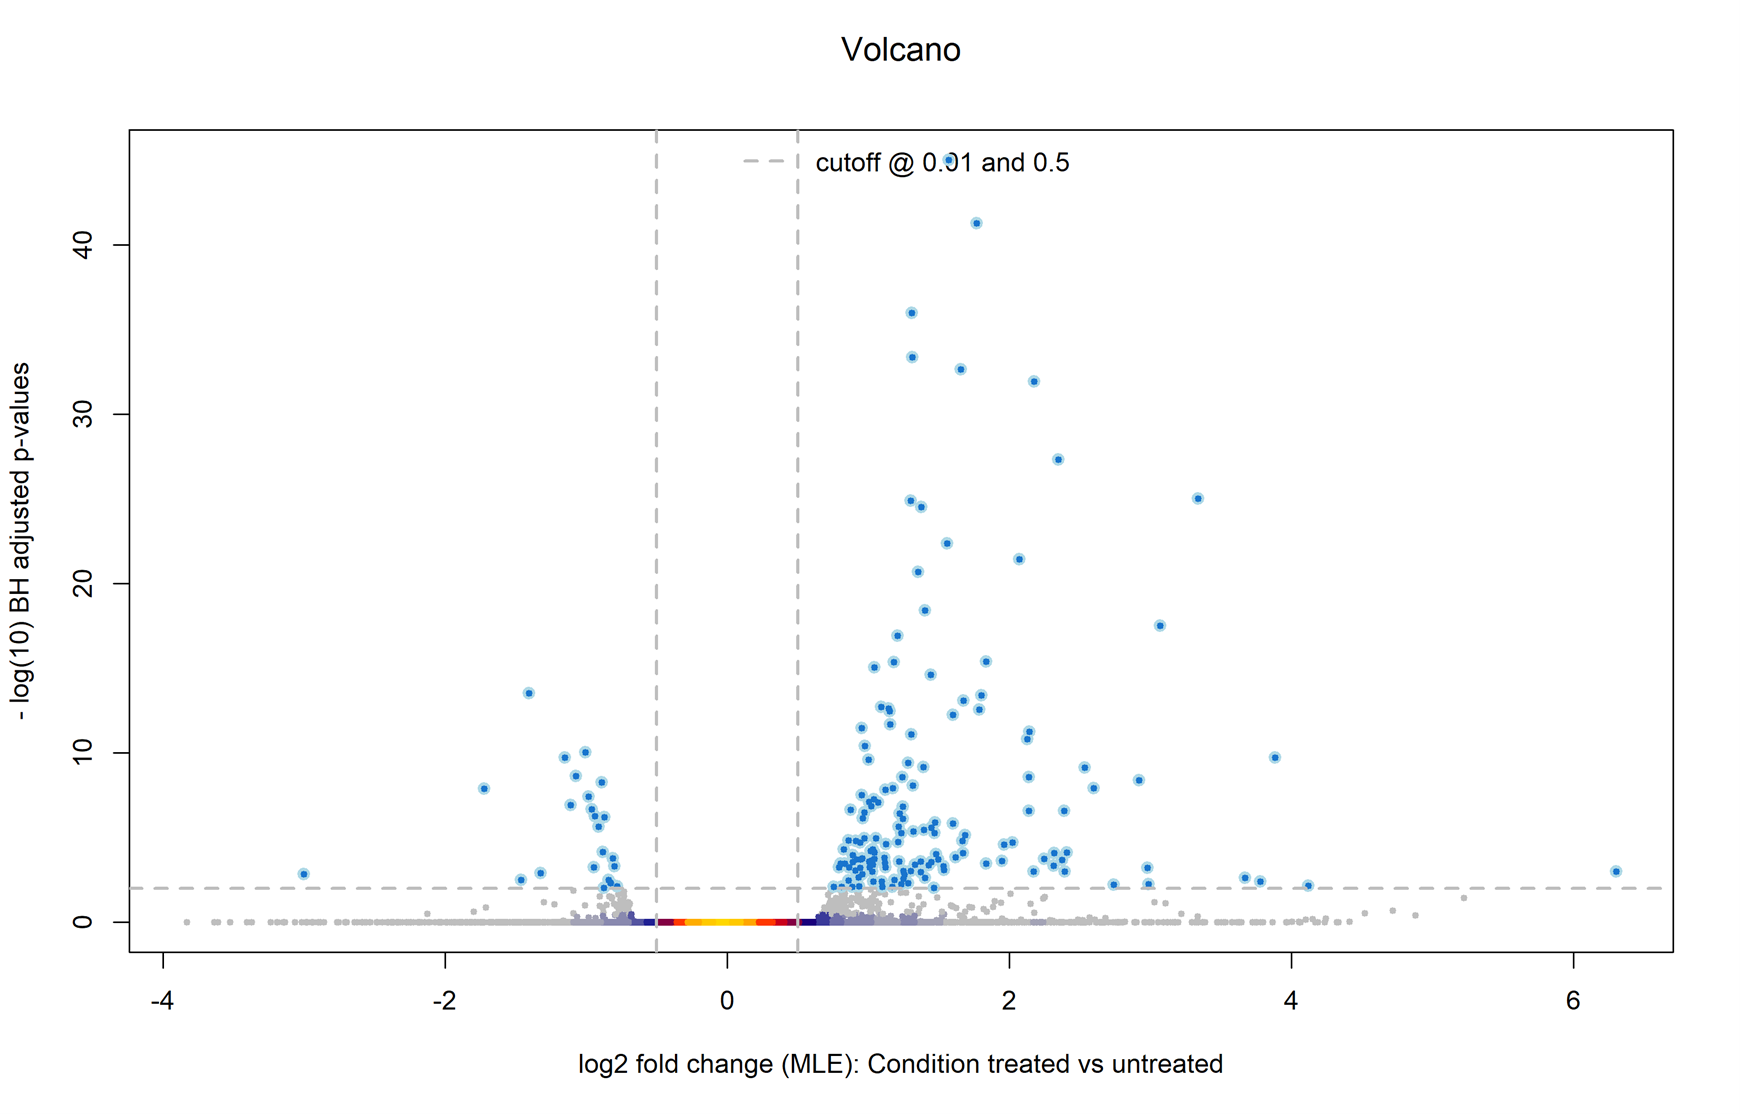
\includegraphics[width=1\linewidth]{07. Chapter 2//Figs/14. rnaseq volcano.png}
    \caption{Enter Caption}
    \label{fig:enter-label}
\end{figure}